%chktex-file 36
%chktex-file 23
%chktex-file 10
%chktex-file 17
%chktex-file 9
%chktex-file 11
%chktex-file 8
\documentclass[computationalMathematics.tex]{subfiles}

\begin{document}

%%%%%%%%%%%%%%~~~~~~~~~~~~~~~~~~~~~~~~~~~~~~~~~~~~~~~~%%%%%%%%%%%%%%%
\section{26th of September 2018 --- F. Poloni}
%%%%%%%%%%%%%%~~~~~~~~~~~~~~~~~~~~~~~~~~~~~~~~~~~~~~~~%%%%%%%%%%%%%%%

\subsection{Orthogonality (II)}
In the previous lecture we introduced some sufficent conditions for matrix orthogonality.

\begin{theorem}
  Let $U \in O(n, \R)$ and let $x \in \R^n$. Then $\norm{Ux} = \norm{x}$.
\end{theorem}

\begin{proof}
  Instead of proving that $\norm{Ux} = \norm{x}$ we will prove $\norm{Ux}^2 = \norm{x}^2$:\\
  
  \[
    \norm{Ux}^2 = \tr{(Ux)} \cdot (Ux) \numeq{(1)} \tr{x} \tr{U} U x = \tr{x} I_n x = \tr{x} x = \norm{x}
  \]

  where $\numeq{(1)}$ follows from the definition of transpose of a product.
\end{proof}

\textbf{Geometrically} an orthogonal transformations (aka matrices) preserve the norm, so an orthogonal matrix $A$ represents a symmetry or a rotation these operations do not alter the size of vectors.

\begin{figure}[H]
    \centering
    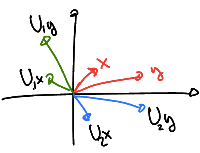
\includegraphics[scale = 2]{pics/26sett/orthgonal.png}
    \caption{Matrix $U_1$ represents a rotation, while $U_2$ is a symmetry operation.}\label{fig:26sett_ortho}
\end{figure}

\begin{definition}[Orthonormality]
  Let $x, y \in R^n$ we say that $x$ and $y$ are \textbf{orthonormal} if $\ps{x}{y} = 0$ and $\norm{x} = \norm{y} = 1$.
\end{definition}

\begin{proposition}
  Let us take $U \in )(n, \R)$.
  Then its columns $U^1, U^2, \ldots, U^n$ are \textbf{orthonormal} and the same holds for its rows.
  \[
  \tr{U^i} U^j = \begin{cases}
    1 \text{ if } i=j\\
    0 \text{ otherwise}
  \end{cases}
  \]
  and
  \[
    U_i \tr{U_j} = \begin{cases}
    1 \text{ if } i=j\\
    0 \text{ otherwise}
  \end{cases}
  \]
\end{proposition}

\begin{proposition}
  The set of orthogonal matrices is closed under product operations.
  Let $U, V \in O(n, \R)$, then $U \cdot V$ is orthogonal.
\end{proposition}

\begin{proof}
  $\tr{(UV)} \cdot (UV) = \tr{V} \tr{U} U V = \tr{V} I_n V = \tr{V} V = I_n$
\end{proof}

Since we will often deal with tall-thin rectangular matrices with
orthonormal columns as $U_1$
  \[
    U_1 = \begin{pmatrix} U^1 & U^2 & \cdots & U^n\end{pmatrix} \in M(m, n, \R) \text{where} m \geq n
  \]
the following fact may come in handy

\begin{proposition}
  $\forall U_1 \in M(m, n, \R)$ where $M \ge n$ and the columns of $u_1$ are orthogonal $\exists U_2$ s.t. $\begin{pmatrix} U_1 & U_2 \end{pmatrix} \in O(m, \R)$.
\end{proposition}

\subsection{Eigenvalues / Eigenvector}

\begin{definition}[Eigenvectors and eigenvalues]
  Let $A \in M(n, \R)$ and let $x \neq 0 \in \R^n$ and $\lambda \in \R$.

  If $Ax = \lambda x$ we say that $x$ is an \textbf{eigenvector} of \textbf{eigenvalue} $\lambda$.
\end{definition}

\begin{theorem}
  Let $A \in M(n, \R)$ (real triangular matrix). The eigenvalues of $A$ are the scalars on the diagonal.
\end{theorem}

\term{
  In this notes we refer to the columns to a generic matrix $A$ as $A^1$ for the first column, $A^2$ for the second column and so on and so forth.

  Conversely, we represent the rows of a matrix $A$ as $A_i$.
}

\begin{definition}[Diagonalizable matrix]
 \emph{Some} matrices $A \in M(n, \R)$ under some conditions can be decomposed as:
\[
  A = V \Lambda \inv{V}
\]
\[
  A = V \Lambda \inv{V} = \begin{pmatrix}
    \\
    V^1 & V^2 & \cdots & V^n\\
    \\
  \end{pmatrix}
  \cdot 
  \begin{pmatrix}
    \lambda_1&&\bigzero\\
    &\lambda_2\\
    &\bigzero& \ddots\\
    &&&\lambda_n\\
  \end{pmatrix}
  \cdot 
  \begin{pmatrix}
    w_1\\
    w_2\\
    \vdots\\
    w_n\\
  \end{pmatrix}
\]

  where $V \in GL(n, \R)$ is the matrix that has as columns the eigenvectors of $A$ $(V^i, \lambda_i)~\forall i=1, \ldots, n$ and $w_i = \inv{V_i}$ are the rows of the inverse of matrix $V$.\\
\end{definition}

\begin{proposition}
  $\forall V^i \in \R$ eigenvectors of $A$ they are still eigenvector of the diagonalized form of $A=V \Lambda \inv{V}$
\end{proposition}

\begin{proof}
  \[
    AV^i = V \Lambda \inv{V} V^i = V \Lambda e_i = \lambda_i V^i
  \]
\end{proof}

Another way to see the diagonalized form of $A$ is the following:
\[
  A = V \Lambda \inv{V} = \sum\limits_{i=1}^{n} v_i\lambda_i w_i^T = 
\]
\[
  \tallthin{$v_1$} \cdot \real{$\lambda_1$} \cdot \shortlarge{$w_1^T$} + \tallthin{$v_2$} \cdot \real{$\lambda_2$} \cdot \shortlarge{$w_2^T$} + \cdots + \tallthin{$v_n$} \cdot \real{$\lambda_n$} \cdot \shortlarge{$w_n^T$}
\]

\syntax{Notice that in Matlab the eigenvalues and eigenvectors of a matrix are computed using the command \texttt{[V, Lambda] = eig(U)} and this operation has a computational complexity of $O(n^3)$.

We can check that the matrix \texttt{A} is equal to the decomposition in this way:
\texttt{A - V*Lambda*inv(V)} or \texttt{norm(A - V*Lambda*inv(V))} (both should be close to zero).}

Notice that not all matrices $A \in M(n, \R)$ allow a diagonal decomposition.
It may happen that such a matrix $A$ is diagonalizable in $\mathds{C}$ and its eigenvalues are complex.

\noindent This decomposition tell us the behavior under repeated application of a matrix $A$ to a vector $x$. This process allow to scale a general vector $x$.\\

\syntax{
e.g \texttt{A = [1 1; 1 1]} and \texttt{x = [ 1 1 ]}\\
then \texttt{A*x} is equal to \texttt{[2 2]'} and \texttt{A*A*x} is equal to \texttt{[4 4]'}
}

\begin{proposition}
  If $A \in M(n, \R)$ is diagonalizable (aka may be written as $A = V \Lambda \inv{V}$) then $A^k x = \sum\limits_{i=1}^{n} \lambda_i^k \alpha_i V^i$, for some $\alpha_i \in \R$.
\end{proposition}

\begin{proof}
  Let us write $x$ in the base of $\R^n$ made of the linearly independent columns of $V$:
  \[
x = V^1 \alpha_1 + V^2 \alpha_2 + \cdots + V^n \alpha_n
  \]
  for some $\alpha_i \in \R$.

 \begin{itemize}
   \item \textsc{Algebraic view point:}
  \begin{equation}
    \begin{split}
      Ax &= A \cdot ( V^1 \alpha_1 + V^2 \alpha_2 + \cdots + V^n \alpha_n)\\
      &= A V^1 \alpha_1 + A V^2 \alpha_2 + \cdots + A V^n \alpha_n\\
      & = \lambda_1 V^1 \alpha_1 + \lambda_2 V^2 \alpha_2 + \cdots + \lambda_n V^n \alpha_n\\
      &= V^1 (\lambda_1 \alpha_1) + V^2 (\lambda_2 \alpha_2) + \cdots + V^n (\lambda_n \alpha_n)\\
    \end{split}
  \end{equation}

  Then
 \begin{equation}
    \begin{split}
      A^2 x &= A \cdot \Big (V^1 (\lambda_1 \alpha_1) + V^2 (\lambda_2 \alpha_2) + \cdots + V^n (\lambda_n \alpha_n) \Big )\\
      &= A V^1 \lambda_1 \alpha_1 + A V^2 \lambda_2 \alpha_2 + \cdots + A V^n \lambda_n \alpha_n\\
      &= {\lambda_1}^2 V^1 \alpha_1 + {\lambda_2}^2 V^2 \alpha_2 + \cdots + A {\lambda_n}^2 V^n \alpha_n\\
    \end{split}
  \end{equation}
The thesis follows inductively.
  
  \item \textsc{Linear algebra view point:}
    \begin{equation}
      \begin{split}
        A^k x &= A \cdot A \cdot \ldots \cdot A \cdot x\\
        &=V \Lambda \cancel{\inv{V}} \cancel{V} \Lambda \cancel{\inv{V}} \ldots \cancel{V} \Lambda \inv{V} x\\
        &= V \Lambda^k \inv{V} x\\
        &=V \begin{pmatrix}
          {\lambda_1}^k\\
          & {\lambda_2}^k\\
          && \ddots\\
          &&&& {\lambda_n}^k\\
        \end{pmatrix}
        \inv{V} x\\
        &=V \begin{pmatrix}
          {\lambda_1}^k\\
          & {\lambda_2}^k\\
          && \ddots\\
          &&&& {\lambda_n}^k\\
        \end{pmatrix}
        \cdot \begin{pmatrix}
          {\alpha_1}\\
          {\alpha_2}\\
          \ddots\\
          {\alpha_n}\\
        \end{pmatrix}
      \end{split}
    \end{equation}

  \end{itemize}
\end{proof}

Notice that if $A$ is not square, $Av$, $\lambda v$ have different sizes and it doesn't make sense to talk about eigenvalues.

\subsubsection{Eigenvector: what could possibly go wrong?}
\begin{enumerate}
    \item  The eigenvalue decomposition is highly non-unique, we can:
    \begin{itemize}
        \item Reorder eigenvalues/vectors
        \item Replace an eigenvector $v_i$ with $2v_i \;,\; −3.5v_i\; \dots$
        \item For matrices with repeated eigenvalues we have even more possibilities:\\
          e.g $I = VIV^{-1}$ for every invertible $V$
    \end{itemize}
    
    \item  some matrices have only complex eigenvalues: e.g. $\begin{pmatrix} 2 & 4\\ -3 & 3\end{pmatrix}$
    
    \item some matrices have fewer eigenvectors than we want and we can't use eigenvalue decomposition: e.g. $\begin{pmatrix} 1 & 1\\ 0 & 1\end{pmatrix}$
    
\end{enumerate}

\noindent Now, thanks to the eigenvalue decomposition we can prove the following:

\begin{theorem}
  Let $A \in M(n, \R)$. If $\abs{\lambda_i} < 1 $ for all eigenvalues $\lambda_i$ of $A$  then $\lim\limits_{k \to \infty} A^k x = 0$.
\end{theorem}

\begin{theorem}
  Let $A \in M(n, \R)$. If $\forall \lambda_i$ eigenvalues of $A$ $\abs{\lambda_i} < \abs{\lambda_1}$ then $A^k x \approx V^1 {\lambda_1}^k \alpha_1$.
\end{theorem}

\begin{proposition}
  Let $A \in M(n, \R)$ be a diagonalizable matrix and let 
  \[
    A=V\Lambda \inv{V} = \begin{pmatrix}
    \\
    V^1 & V^2 & \cdots & V^n\\
    \\
  \end{pmatrix}
  \cdot 
  \begin{pmatrix}
    \lambda_1\\
    &\lambda_2\\
    && \ddots\\
    &&&&&\lambda_n\\
  \end{pmatrix}
  \cdot 
  \begin{pmatrix}
    w_1\\
    w_2\\
    \vdots\\
    w_n\\
  \end{pmatrix}
\]

  Let us now consider a reordering of $V$'s columns and apply the same permutation to the ``diagonal vector'' of $\Lambda$ such that
  
\[
    \hat{V} = \begin{pmatrix}
    \\
    V^2 & V^1 & V^3 \cdots & V^n\\
    \\
  \end{pmatrix}
  \text{ and }
  \hat{\Lambda}= \begin{pmatrix}
    \lambda_2\\
    &\lambda_1\\
    &&\lambda_3\\
    &&& \ddots\\
    &&&&&&\lambda_n\\
  \end{pmatrix}
\]

  A can be diagonalized through such $\hat{V}$ and $\hat{\Lambda}$ as $A = V \Lambda \inv{V} = \hat{V} \hat{\Lambda} \inv{\hat{V}}$.
\end{proposition}

Moreover, in the case of repeated eigenvalues

\begin{proposition}
  Let $A \in M(n, \R)$ a diagonalizable matrix such that $A = V \Lambda \inv{V}$, where $\lambda_1 = \lambda_2$ (without loss of generality). Then $V$ can be replaced by $\widetilde{V} = \begin{pmatrix}
    \\
    \\
    V^1 + V^2 & V^1 - V^2 & V^3 & \cdots & V^n\\
    \\
    \\
  \end{pmatrix}$.
\end{proposition}

\begin{theorem}[Spectral theorem]
  Let $A \in S(n, \R)$ ($A$ is a real symmetric matrix). Then $A$ is diagonalizable $A = U\Lambda \inv{U}$, where eigenvalues are all real numbers and we can take $U$ orthogonal matrix.
\end{theorem}


Notice that for symmetric matrices none of the ``unlucky'' situations enumerated above may happen (it is justified by the spectral theorem).

\syntax{
If we have an symmetric matrix \texttt{B} and we compute \texttt{[V, D] = eig(B)}, matlab will always return an orthogonal matrix $V$.
}

\begin{definition}[Quadratic form]
  Let $Q \in S(n, \R)$ we define \textbf{quadratic form}
  \[
    f(x) = \tr{x} Q x
  \]
  for each $x \in \R^{n}$.
\end{definition}

Geometrically, a quadratic form defines a paraboloids.

\begin{example}
  Let $f_1(\begin{pmatrix} x_1\\ x_2 \end{pmatrix}) = \begin{pmatrix} x_1 & x_2 \end{pmatrix} \begin{pmatrix} 3 & 2 \\ 2 & 4 \end{pmatrix}\begin{pmatrix} x_1\\ x_2 \end{pmatrix} = 3 {x_1}^2 + 4 x_1 x_2 + 4 {x_2}^2$ and let $f_2(\begin{pmatrix} x_1\\ x_2 \end{pmatrix}) = \begin{pmatrix} x_1 & x_2 \end{pmatrix} \begin{pmatrix} 3 & 2 \\ 2 & -4 \end{pmatrix}\begin{pmatrix} x_1\\ x_2 \end{pmatrix} = 3 {x_1}^2 + 4 x_1 x_2 -4 {x_2}^2$

For a graphic hint see \Cref{fig:26sett_quadratic}.

\begin{figure}[h!]
	\centering\scriptsize
	\hspace*{\fill}
  \subfigure[$f_1(x)$]{
		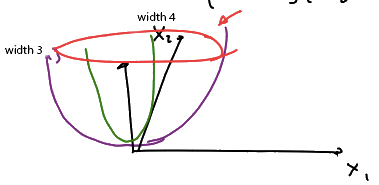
\includegraphics[scale=.5]{pics/26sett/quadratic_form_1.png}\label{subfig:quad1}
	} \hfill
  \subfigure[$f_2(x)$]{
		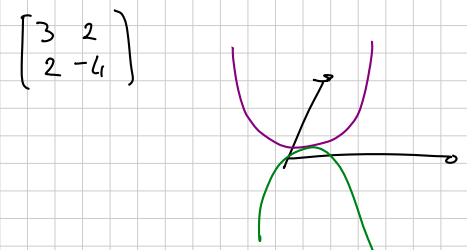
\includegraphics[scale=2]{pics/26sett/quadratic_form_2.png}\label{subfig:quad2}
	} \hspace*{\fill}
	\caption{The plot of functions.}\label{fig:26sett_quadratic}
\end{figure}

\end{example}

\begin{proposition}
  Let $Q \in S(n, \R)$ (For a fixed symmetric matrix) and let $x \in \R^n$. Then 
  \[
    \lambda_{\text{min}} \sqrnorm{x} \le \tr{x}Qx \le \lambda_{\text{max}} \sqrnorm{x}
  \]
  where $\lambda_{\text{max}}$ and $\lambda_{\text{min}}$ are respectively the eigenvalue of maximum value and the eigenvalue of minimum value.
\end{proposition}

\begin{proof}
  \begin{description}
    \item[{\sc Easy case with $Q$ diagonal:}]
    
      \[\tr{x}Qx = \tr{x} \cdot \begin{pmatrix}
    \lambda_2\\
    &\lambda_1\\
    &&\lambda_3\\
    &&& \ddots\\
    &&&&&&\lambda_n\\
    \end{pmatrix}
      \cdot x = \lambda_1 {x_1}^2 + \lambda_2 {x_2}^2 + \cdots + \lambda_n {x_n}^2
      \]
  It is obvious that this sum is bounded by:
  \[
    \lambda_{\text{min}} \cdot ({x_1}^2 +{x_2}^2 + \cdots + {x_n}^2) \le  \lambda_1 {x_1}^2 + \lambda_2 {x_2}^2 + \cdots + \lambda_n {x_n}^2 \le \lambda_{\text{max}} \cdot ({x_1}^2 +{x_2}^2 + \cdots + {x_n}^2)
  \]

   The following holds: $ \lambda_{\text{min}} \cdot ({x_1}^2 +{x_2}^2 + \cdots + {x_n}^2) =  \lambda_{\text{min}} \cdot \tr{x} x =  \lambda_{\text{min}} \cdot \sqrnorm{x}$ and, on the other hand, $ \lambda_{\text{max}} \cdot ({x_1}^2 +{x_2}^2 + \cdots + {x_n}^2) =  \lambda_{\text{max}} \cdot \tr{x} x =  \lambda_{\text{max}} \cdot \sqrnorm{x}$ and this proves the fact in the special case of diagonal matrix $Q$.
    \item[{\sc General case:}]
      Let us represent $Q$ through its eigendecomposition: $A = U \Lambda \inv{U} = U \Lambda \tr{U}$, where $U$ is an orthogonal matrix.
      \[
        \tr{x}Qx = \tr{x} U \Lambda \tr{U} x \numeq{(1)} \tr{y} \Lambda y
      \]

      where $\numeq{(1)}$ is due to the change of variable $y = \tr{U} x$ (that implies $\tr{y} = \tr{x} U$).

      By the same argument used in the diagonal case,
      \[
        \lambda_{\text{min}} \cdot \sqrnorm{y} \le \tr{y} \Lambda y \le \lambda_{\text{max}} \cdot \sqrnorm{y}
      \]
      Now the point is that if we can replace $\sqrnorm{\tr{U}x} = \sqrnorm{y}$ with $\sqrnorm{x}$ we have proved the theorem.
      In fact this is true, due to the orthogonality of matrix $U$ and \Cref{fact:20sett}.
  \end{description}
\end{proof}

\begin{corollary}
  Let $Q \in S(n, \R)$ and let $x \in \R^n$. If $x \neq 0$, $\lambda_{\text{min}} \le \frac{\tr{x}Qx}{\sqrnorm{x}} \le \lambda_{\text{max}}$, where $\lambda_{\text{max}}$ and $\lambda_{\text{min}}$ are respectively the eigenvalue of maximum value and the eigenvalue of minimum value.
\end{corollary}

\begin{definition}[Positive semidefinite]
  Let $Q \in S(n, \R)$. We say that $Q$ is \textbf{positive semidefinite} (and we indicate $\succeq 0$) if 
  \[
    \tr{x} Q x \ge 0\norm{x}^2 \geq 0
  \]
\end{definition}

\begin{definition}[Positive definite]
   Let $Q \in S(n, \R)$. We say that $Q$ is \textbf{positive definite} (and we indicate $\succ 0$) if 
  \[
    \tr{x} Q x \ge 0\norm{x}^2 > 0
  \]
\end{definition}

\begin{proposition}
  Let $Q \in S(n, \R)$. The following holds
  
  \[
    Q \text{ is positive semidefinite} \iff \forall \lambda \text{ eigenvalue of } Q ~ \lambda \ge 0
  \]

  And this holds with the $>0$ in the positive definite case.
\end{proposition}

\begin{proof}~\\

  \indent ($\Leftarrow$) $\tr{x} Q x \ge \lambda_{\text{min}} \geq 0$ since we are in the hypothesis that all the eigenvalues are $\geq 0$

  \indent  ($\Rightarrow$) $ \forall v_i$ eigenvector of $Q$ $0 \le \tr{v_i} A v_i = \tr{v_i} \cdot ( \lambda_i v_i) = \lambda_i  \tr{v_i} v_i = \lambda_i \sqrnorm{v_i} \Rightarrow \lambda_i \ge 0$.
\end{proof}

\begin{corollary}
  Let $Q \in S(n, \R)$ such that $Q \succeq 0$. The following holds:
  \[
    A \text{ is invertible} \iff Q \text{ is strictly positive definite}
  \]
\end{corollary}

\begin{proposition}
  Let $B \in M(m, n, \R)$ (possibly rectangular), $\tr{B} B \in S(n, \R)$ is a valid product and it is a square, symmetric, positive semidefinite matrix.
\end{proposition}

\begin{proof}
\begin{description}
  \item[{\sc Symmetry:}] $\tr{(\tr{B}B)} = \tr{B} \cdot \tr{(\tr{B})} = \tr{B} B$.
  \item[{\sc Positive definite:}] $\tr{x} \tr{B} B x = \tr{(B x)} (Bx) = \sqrnorm{Bx} \ge 0$
\end{description}
\end{proof}

\begin{corollary}
  The same holds for $B\tr{B} \in S(m, \R)$ and it is easily proved taking $C = \tr{B} \in M(n, m, \R)$.
\end{corollary}
\syntax{
  In ordert to check if a matrix $A$ is positive definite in Matlab we can look at its eigenvalues (cfr. \texttt{eig(A)}).
}

Notice that in the \textbf{complex} case most of these properties work as well, but it is needed to replace $A^T$ with $\overline{A^T}$\footnote{Often denoted with $A^*$ or $A^H$ and called \textbf{Hermitian matrix}.} (transpose and entrywise conjugate).

\noindent The norm of a complex vector is computed as
\[
  \norm{x}_2^2 = x^*x = \overline{x_1}x_1 + \overline{x_2}x_2 + \dots + \overline{x_n}x_n = \abs{x_1}^2 + \dots + \abs{x_n}^2 \in \R^+ \cup \{0\}
\]

\noindent Moreover, in the complex case, $UU^* = I$ is called \textbf{unitary matrix} (orthogonal + complex)

\end{document}
